%----------------------------------------------------------------------------------------
%   Доорх хэсгийг өөрчлөх шаардлагагүй
%----------------------------------------------------------------------------------------
%!TEX TS-program = xelatex
%!TEX encoding = UTF-8 Unicode
\documentclass[12pt,A4]{report}

\usepackage{fontspec,xltxtra,xunicode}
\setmainfont[Ligatures=TeX]{Times New Roman}
\setsansfont{Arial}

% \usepackage[utf8x]{inputenc}
% \usepackage[mongolian]{babel}
%\usepackage{natbib}
\usepackage{geometry}
%\usepackage{fancyheadings} fancyheadings is obsolete: replaced by fancyhdr. JL
\usepackage{fancyhdr}
\usepackage{float}
\usepackage{afterpage}
\usepackage{graphicx}
\usepackage{amsmath,amssymb,amsbsy}
\usepackage{dcolumn,array}
\usepackage{tocloft}
\usepackage{dics}
\usepackage{nomencl}
\usepackage{upgreek}
\newcommand{\argmin}{\arg\!\min}
\usepackage{mathtools}
\usepackage[hidelinks]{hyperref}

\usepackage{algorithm}
\usepackage{algpseudocode}

\usepackage{listings}
\DeclarePairedDelimiter\abs{\lvert}{\rvert}%
\makeatletter
\usepackage{caption}
\captionsetup[table]{belowskip=0.5pt}
\usepackage{subfiles}

\usepackage{listings}
\renewcommand{\lstlistingname}{Код}
\renewcommand{\lstlistlistingname}{\lstlistingname ын жагсаалт}

\usepackage{color}
\definecolor{codegreen}{rgb}{0,0.6,0}
\definecolor{codegray}{rgb}{0.5,0.5,0.5}
\definecolor{codepurple}{rgb}{0.58,0,0.82}
\definecolor{backcolour}{rgb}{0.99,0.99,0.99}
 
\lstdefinestyle{mystyle}{
    basicstyle=\ttfamily\small,
    backgroundcolor=\color{backcolour},   
    commentstyle=\color{codegreen},
    keywordstyle=\color{magenta},
    numberstyle=\tiny\color{codegray},
    stringstyle=\color{codepurple},
    %basicstyle=\footnotesize,
    breakatwhitespace=false,         
    breaklines=true,                 
    captionpos=b,                    
    keepspaces=false,                 
    numbers=left,                    
    numbersep=10pt,                  
    showspaces=false,                
    showstringspaces=true,
    showtabs=false,                  
    tabsize=2
}
 
\lstset{style=mystyle, label=DescriptiveLabel} 

\let\oldabs\abs
\def\abs{\@ifstar{\oldabs}{\oldabs*}}
\makenomenclature
\begin{document}


%----------------------------------------------------------------------------------------
%   Өөрийн мэдээллээ оруулах хэсэг
%----------------------------------------------------------------------------------------

% Дипломийн ажлын сэдэв
\title{Урамшууллын системийн цогц хөгжүүлэлт}
% Дипломын ажлын англи нэр
\titleEng{Full stack loyalty system developing}
% Өөрийн овог нэрийг бүтнээр нь бичнэ
\author{Нямдоржын Энхболд}
% Өөрийн овгийн эхний үсэг нэрээ бичнэ
\authorShort{Н.Энхболд}

% СиСи дугаар 
\sisiId{20B1NUM0102}
% Их сургуулийн нэр
\university{МОНГОЛ УЛСЫН ИХ СУРГУУЛЬ}
% Бүрэлдэхүүн сургуулийн нэр
\faculty{ХЭРЭГЛЭЭНИЙ ШИНЖЛЭХ УХААН, ИНЖЕНЕРЧЛЭЛИЙН СУРГУУЛЬ}
% Тэнхимийн нэр
\department{МЭДЭЭЛЭЛ, КОМПЬЮТЕРИЙН УХААНЫ ТЭНХИМ}
% Зэргийн нэр
\degreeName{Үйлдвэрлэлийн дадлагын тайлан}
% Суралцаж буй хөтөлбөрийн нэр
\programeName{Програм хангамж (D061302)}
% Хэвлэгдсэн газар
\cityName{Улаанбаатар}
% Хэвлэгдсэн огноо
\gradyear{2023 оны 09 сар}

%----------------------------------------------------------------------------------------
%   Доорх хэсгийг өөрчлөх шаардлагагүй
%----------------------------------------------------------------------------------------
%----------------------Нүүр хуудастай хамаатай зүйлс----------------------------
\pagenumbering{roman}
\makefrontpage
\maketitle

\doublespace

% Decleration
\begin{huge}
\textbf{Зохиогчийн баталгаа}
\end{huge} \\ \ \\ 
\doublespace
Миний бие \@author \ "\@title" \ сэдэвтэй судалгааны ажлыг гүйцэтгэсэн болохыг зарлаж дараах зүйлсийг баталж байна:
\begin{itemize}
\item Ажил нь бүхэлдээ эсвэл ихэнхдээ Монгол Улсын Их Сургуулийн "Үйлдвэрлэлийн дадлага (INTE401)" хичээлийг тооцуулахаар дэвшүүлсэн болно.
\item Энэ ажлын аль нэг хэсгийг эсвэл бүхлээр нь ямар нэг их, дээд сургуулийн зэрэг горилох, хичээл тооцуулахаар оруулж байгаагүй.
\item Бусдын хийсэн ажлаас хуулбарлаагүй, ашигласан бол ишлэл, зүүлт хийсэн.
\item Ажлыг би өөрөө (хамтарч) хийсэн ба миний хийсэн ажил, үзүүлсэн дэмжлэгийг дипломын ажилд тодорхой тусгасан. 
\item Ажилд тусалсан бүх эх сурвалжид талархаж байна. 
\end{itemize} 
\ 

Гарын үсэг: \underline{\hspace{5cm}} 

Огноо: 	\ \ \underline{\hspace{3cm}}

% Гарчгийг автоматаар оруулна
\setcounter{tocdepth}{1}
\tableofcontents

% Зургийн жагсаалтыг автоматаар оруулна
\listoffigures

% Хүснэгтийн жагсаалтыг автоматаар оруулна
\listoftables

% Кодын жагсаалтыг автоматаар оруулна
\lstlistoflistings

% This puts the word "Page" right justified above everything else.
\newpage
%% \addtocontents{lof}{Зураг~\hfill Хуудас \par}
\newpage
%% \addtocontents{lot}{Хүснэгт~\hfill Хуудас \par}

\renewcommand{\cftlabel}{Зураг}


\doublespace
\pagenumbering{arabic}


% Удиртгалыг оруулж ирэх ба abstract.tex файлд удиртгалаа бичнэ
\begin{abstract}
  
  
  Миний бие Н. Энхболд нь үйлдвэрлэлийн дадлагын хугацааны хүрээнд "MOGUL" группийн салбар компани болох "Nomadic Software Solution" ХХК-д хөгжүүлэгчдийн ашигладаг технологиудыг судалж, сурсан мэдлэгээрээ HPoint төслийг эхлүүлсэн бөгөөд нийт 5 хүний бүрэлдэхүүн бүхий багийг ахлаж төслийг эхний байдлаар хэрэгжүүлсэн билээ. 

  HPoint төслийн гол зорилго нь "Hoome" платформд урамшууллын програмыг нэвтрүүлснээр хэрэглэгчдийн тоог үнэмлэхүйц байдлаар өсгөх юм.

  Төслийн баг нь архитектор, back-end хөгжүүлэгч, програм хангамж хөтөлбөрийн 2 дадлагын оюутнуудаас бүрдэх бөгөөд төслийн хүрээнд мобайл хөгжүүлэлт, микросервис хөгжүүлэлт, өгөгдлийн сангийн зохиомж, хэрэглэгчийн интерфейсийн зохиомж зэрэг ажлууд өрнөсөн болно.

  Үйлдвэрлэлийн дадлагын хугацаанд эдгээр ажлуудад ашиглагдах технологиудыг судалж, хэрэгжүүлэлтүүдийг гүйцэтгэсэн билээ.
\end{abstract}


\chapter{Төлөвлөгөө}
\begin{table}[h]
\caption{Үйлдвэрлэлийн дадлагын төлөвлөгөө}
\begin{tabular}{|p{0.5cm}|p{8cm}|l|l|p{2.5cm}|}
\hline
\textbf{№} & \textbf{Гүйцэтгэх ажил} & \textbf{Хугацаа} & \textbf{Төлөв} & \textbf{Удирдагчийн үнэлгээ} \\ \hline
1 & Spring boot технологи болон JHipster-ийн талаар судлах & 1 өдөр & Гүйцэгтэсэн & 10/10 \\ \hline
2 & Keycloak технологийн талаар судлах & 1 өдөр & Гүйцэгтэсэн & 10/10 \\ \hline
3 & Өмнө хөгжүүлэгдсэн микросервис дээр feature нэмэх & 3 өдөр & Гүйцэгтэсэн & 10/10 \\ \hline
4 & Flutter-ийн BLoC технологийн талаар судлах & 1 өдөр & Гүйцэгтэсэн & 10/10 \\ \hline
5 & Hoome мобайл аппликейшн дээр зогсоолын төлбөр төлөх хэсэг дээр bug засах, карт холбох feature нэмэх & 4 өдөр & Гүйцэгтэсэн & 10/10 \\ \hline
6 & Hoome платформын хэрэглэгчийн тоог өсгөх шийдэл олох, зохиомжийг гаргах & 1 өдөр & Гүйцэгтэсэн & 10/10 \\ \hline
7 & Микросервис хөгжүүлэлтийг хийх API endpoint-уудыг бэлдэх (Багаар) & 6 өдөр & Гүйцэгтэсэн & 10/10 \\ \hline
8 & "Hoome" мобайл аппликейшн дээр шийдлээ оруулж өгөх, дизайныг хэрэгжүүлэх & 2 өдөр & Гүйцэгтэсэн & 10/10 \\ \hline
9 & Микросервис дээр integration тест бичих & 2 өдөр & Гүйцэгтэсэн & 10/10 \\ \hline
\end{tabular}
\end{table}

%----------------------------------------------------------------------------------------
%   Дипломын үндсэн хэсэг эндээс эхэлнэ
%----------------------------------------------------------------------------------------
%\addcontentsline{toc}{part}{БҮЛГҮҮД}
% Шинэ бүлэг
% \subfile{writing.tex}
\chapter{Байгууллагын тухай}

\hspace{0.5cm}
"MOGUL" групп нь 1997 онд компьютер, компьютерийн тоног төхөөрөмж нэвтрүүлэх, үйлчилгээ үзүүлэх зорилгоор үйл ажиллагаагаа эхэлж байсан бөгөөд Мэдээллийн Технологийн чиглэлээр төрөлжин үйл ажиллагаа явуулдаг 6 компанитайгаар 26 дахь жилдээ ажиллаж байгаа. Нийт 380 гаруй ажилтан, тэдгээрийн 200 гаруй ажилтан нь инженерүүд байдаг. Мэдээллийн технологийн дэд бүтэц, тоног төхөөрөмжийн худалдаа, үйлчилгээ, Мэдээллийн болон биет аюулгүй байдал, Программ хангамж үйлдвэрлэл, Цахим засаг, Клауд болон Менежед үйлчилгээ, Дата болон AI, салбаруудын мэдээллийн технологийн шийдэл чиглэлээр үйл ажиллагаа явуулдаг.

\section{Компаний тухай}
"MOGUL" групп нь 2023 оны өвлийн улиралд 6 салбар компанитай байсан бөгөөд эдгээрт: 
\begin{itemize}
	\item ITZone ХХК
	\item Новелсофт ХХК
	\item Могул Сервис энд Саппорт ХХК
	\item Дижитал Воркс ХХК
	\item Дижитал Повер ХХК
	\item Могул Экспресс ХХК
\end{itemize}
компаниуд орно. "Новелсофт" ХХК-ийн бизнесийн үйл ажиллагаа өргөжсөнөөр "Nomadic Software Solution" ХХК компанийг 2023 оны хаврын улирал үүсгэн байгуулсан. 

\section{Үйл ажиллагаа}
"Новелсофт" ХХК нь захиалгат програм хангамж хөгжүүлэлт, дата аналитик, дата менежмент, мэргэжлийн үйлчилгээ (outsourcing) зэрэг үйл ажиллагаа явуулдаг байсан ба үүнээс програм хангамж болон дата аналитик гэх үйл ажиллагааны хүрээнд 2 хуваагдан "Nomadic SS" ХХК бий болсон. 

"Nomadic SS" ХХК нь одоогоор програм хангамж хөгжүүлэлт, мэргэжлийн үйлчилгээ (outsourcing) зэрэг үйл ажиллагааг явуулдаг.

\section{Технологиуд болон системүүд}
Компаний хувьд хөгжүүлэгдэж буй системүүд нь цогц системүүд байдаг ба дийлэнх хөгжүүлэгчдийн туршлага, системийн зохиомжоос хамааран
\begin{itemize}
	\item Front-end
	\begin{itemize}
		\item Mobile: Flutter - BLoC (Business Logic Components)
		\item Web: Angular - Primeng
		\item Desktop: .NET
	\end{itemize}
	\item Server
	\begin{itemize}
		\item Java - JHipster Spring boot
		\item OAuth - Keycloak
		\item Cassandra
		\item Kafka
		\item Redis
		\item Prometheus
	\end{itemize}
\end{itemize} 
технологиудыг best practice болгон мөрдөж ашигладаг. Хэрэглэгчийн шаардлагаас үүдэн өөр технологиудыг ашигласан тохиолдлууд ч байдаг.

\chapter{Hoome төсөл}

\hspace{0.5cm}
Үйлдвэрлэлийн дадлагын хүрээнд одоо идэвхитэй явагдаж буй "Hoome" төсөл дээр ажилласан бөгөөд энэхүү төсөл нь Hoome мобайл аппликейшн, Hoome сөх веб, Hoome контор веб зэрэг системүүдээс бүрдэх цогц систем юм. Одоогоор бүртгэлтэй 24000 хэрэглэгч байгаа ба тэдгээрийн 13000 нь идэвхитэй хэрэглэгч. 

Бизнесийн үйл ажиллагаа нь голчлон хэрэглэгчдийн өдөр тутмын амьдрал дээр тулгуурласан бөгөөд СӨХ-өөс гадна машины зогсоолын хэсгийг нэвтрүүлээд байгаа билээ. Зогсоолын хэсэг нь бие даасан систем бөгөөд CCP(Cloud Car Parking) гэх төслийн хүрээнд идэвхитэй хэрэгжиж байгаа болно. Уг системийг "Hoome" мобайл аппликейшнд feature байдлаар оруулж өгсөн байгаа. 

"Novelsoft" ХХК-ийн бүтээгдэхүүн болох "Homebook" СӨХ-ийн системийг сайжруулж сошиал коммунити аппликейшн болгож 2022 онд улмаар "Hoome" гэх шинэ төслийг эхлүүлсэн. 


% Бүлгийн дэд гарчиг
\section{Хотхон}
"Hoome" платформын хотхоны систем нь СӨХ-ийн менежмент, төлбөр, оршин суугчдын бүх төрлийн харилцааг удирдах тусгай систем болон түүнийг иргэдэд хүргэх "Hoome" сошиал аппын цогц бөгөөд
\begin{itemize}
  \item СӨХ-ийн төлбөр бодолт
  \item Хэрэглэгчийн төлбөр төлөлт
  \item Автомат иБаримт гаргах, илгээх
  \item Тайлан гаргах
  \item Хотхоны бүлгэм үүсгэх, сошиал пост, чат
  \item Оршин суугчдын жагсаалт, мэдээлэл, автомат бүртгэл
  \item Зогсоол, агуулах удирдлага
\end{itemize}
зэрэг функцуудээс бүрдэнэ.

\section{Контор}
"Hoome" платформын хотхоны систем нь конторын төлбөр бодолт, үйлчилгээний захиалга авах гэх мэт бүх үйл ажиллагааг удирдах, системтэй.
\begin{itemize}
  \item Бүх хэрэглэгчийн жагсаалт
  \item Конторын төлбөр бодолт
  \item Хэрэглэгчийн төлбөр төлөлт
  \item Тайлан гаргах
  \item Тоолуурын заалт
  \item Тариф удирдлага тохиргоо
  \item Автомат иБаримт гаргах, илгээх
\end{itemize}
зэрэг функцуудээс бүрдэнэ.

\section{Мобайл аппликейшн}
"Hoome" платформын мобайл аппликейшн нь СӨХ-ийн төлбөр төлөгч болон Hoome-д бүртгэлтэй зогсоолд машинаа тавьсан хэрэглэгчдэд зориулагдсан. Хэрэглэгч өөрийн хотхоны СӨХ-д элссэнээр сар бүрийн төлөх зардлууд болон тооцоог нэг дороос харах боломжтой болно. Зогсоолын төлбөр буюу "Cloud Car Parking" систем нь Hoome-д бүртгэлтэй зогсоолууд дээр машин тавьсан хэрэглэчийг төлбөрийг орсон хугацаанаас нь бодож тооцдог бөгөөд давхар orgware буюу хаалгач хүнийг ажиллуулдаг билээ. Тухайн зогсоолын төлбөрийг зөвхөн "Hoome" биш, зарим тохиолдолд "Toki" аппликейшнийн хэрэглэгчид аппликейшнээрээ дамжуулан төлбөрөө төлдөг бөгөөд энэ нь Hoome-CCP-ийн зэрэгцээ орших ижил төстэй систем болно.

Энэхүү асуудлыг шийдэхээр шийдэл дэвшүүлж дадлагын хугацаанд "Hoome" платформын front-end болон back-end хөгжүүлэлтүүдийг хийж гүйцэтгэсэн билээ. 

\begin{figure*}[ht!]
  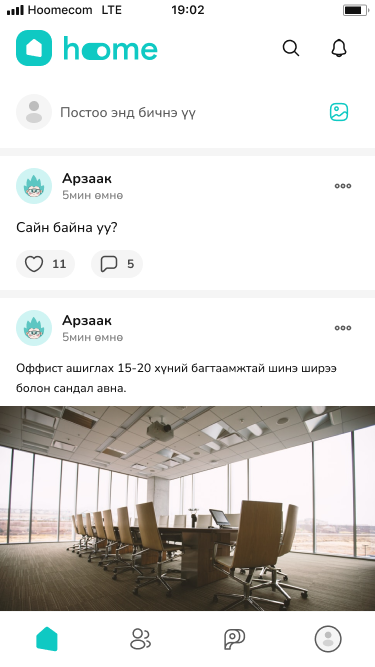
\includegraphics[width=.4\textwidth]{imgs/Home.png}\hfill
  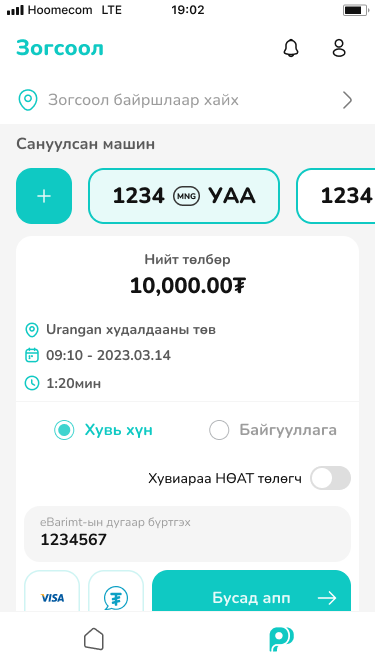
\includegraphics[width=.4\textwidth]{imgs/Parkly.png}
  \caption{Hoome - Коммунити нүүр.}
  \caption{Hoome - Cloud Car Parking нүүр.}
\end{figure*}

\chapter{Ишлэл, зүүлт}
\section{Ишлэл}
Ашигласан материал эсвэл номзүйг бичвэр тодор ишлэхдээ cite командаар заалтыг нь оруулна. 
Үүний тулд энэ хуудасны хамгийн доор байгаа \textit{Ашигласан материал, ном зүй} хэсэгт 
bibitem командыг нэмнэ. \\


Жишээ нь: bibitem\{image1\} Гарчиг, Зохиогчдын нэр, хэвлэсэн он, хэвлэсэн газар

Дээрх жишээнд image1 гэдэг нь ишлэх нэр. Доод талын мөрөнд нь байгаа дарааллын дагуу 
ашигласан материалыг бичнэ. 

Ишлэхдээ cite командад ишлэх нэрийг дамжуулж өгнө. Жишээ нь cite\{image1\}.
\section{Зүүлт}
Зүүлтийг footnote командаар оруулна \footnote{Энэ холбоосоос зүүлтийн талаар дэлгэрэнгүй унш: \url{https://www.sharelatex.com/learn/Footnotes}}. 

\chapter{Зураг}
Зураг оруулахдаа includegraphics командыг ашиглана. Доорх жишээнд figure01.png гэдэг нь зургийн файлын нэр бөгөөд өргөтгөлийг заавал бичих шаардлагагүй. Зургийн файл нь main.tex файлтай нэг фолдерт байх шаардлагатайг анхаарна уу! Дэлгэрэнгүйг \cite{image1}-с үз.


\includegraphics{figure01.png}


\section{Зургийн хэмжээ өөрчлөх}
Хэмжээг томруулахдаа 0-1 хооронд утга ашиглана. Хэрэв 2 гэвэл 2 дахин томроно. 
\begin{center}
includegraphics[scale=0.5]\{figure01\} 
\end{center}


\includegraphics[scale=0.9]{figure01}

Өндөр өргөнийг шууд зааж өгч болох бөгөөд дөрвөлжин хаалтан дотор доорх байдлаар бичнэ. 
\begin{center}
includegraphics[width=3cm, height=4cm]\{figure01\}
\end{center}

\includegraphics[width=3cm, height=4cm]{figure01}

\section{Зураг эргүүлэх}
Зургийн эргүүлэхдээ angle параметрт эргүүлэх өнцгийн хэмжээг өгнө. 
\begin{center}
includegraphics[width=3cm, height=4cm, angle=45]\{figure01\}
\end{center}

\includegraphics[width=3cm, height=4cm, angle=45]{figure01}

\section{Зургийн нэр}
Зургын нэрийг begin\{figure\} хооронд includegraphics командтай хамт оруулна Зураг \ref{fig:lion1}-ыг хар. 

Энд зургийн нэрээс гадна label-ийг давхар бичиж өгөх шаардлагатай ба энэ нь зургийн дугаараар заалт хийхэд ашиглана. Жишээ нь: Зураг \ref{fig:lion2}

\begin{figure}[h]
\centering

\includegraphics[scale=0.9]{figure01}
\caption{Зураг голлуулах}
\label{fig:lion1}
\end{figure}

\section{Зураг голлуулах}
Зургийг голлуулахдаа includegraphics командын өмнө centering 
командыг бичээд reflectbox командыг includegraphics болон caption 
командуудад үйлчлэхээр оруулна.
	
\begin{figure}[h]
		
\includegraphics[scale=0.5]{figure01.png}
    	\caption{Зургийн нэрийг энд бичнэ}
	    
\label{fig:lion2}
\end{figure}

\section{Зургийн чанар}
LaTex-т зургийг вектор форматаар (svg, eps) оруулбал хэвлэх болон томруулж харахад зургийн чанар 
алдагдахгүй. Тиймээс аль болох вектор зураг оруулж өгвөл зүгээр. 

\chapter{Хүснэгт оруулах}
Хүснэгт оруулахад tabular командыг ашигладаг \cite{table}. 

\begin{table}[h]
\centering
\caption{Хүснэгтийн нэр. Хүснэгтийн нэр хүснэгтийн дээд талд байрлана. }
\label{my-label}
\begin{tabular}{|l|l|l|l|l|}
\hline
\textbf{Багана1} & \textbf{Багана2}  & \textbf{Багана3} & \textbf{Багана4} & \textbf{Багана5} \\ \hline
өгөгдөл          & \textit{өгөгдөл1} &                  &                  &                  \\ \hline
                 &                   &                  &                  &                  \\ \hline
                 &                   &                  &                  &                  \\ \hline
\end{tabular}
\end{table}

\section{Хүснэгт зурах хэрэгсэл}
Цэвэр LaTex кодоор Хүснэгт үүсгэхэд харьцангуй төвөгтэй байдаг учир 
хялбар хэрэгслийг ашиглаж болно. 

Тухайлбал \url{https://www.tablesgenerator.com/} холбоосруу орж хүснэгтийг визуал орчинд зураад үүсгэж өгсөн LaTex кодыг энд хуулж оруулна. 

\chapter{Код ба алгоритм оруулах}
Код оруулахдаа begin\{lstlisting\}  ... end\{lstlisting\} командын хооронд бичнэ.

\begin{lstlisting}[language=C, caption=С хэлний кодын жишээ, frame=single]
#include <stdio.h>
#define N 10
/* Block
 * comment */
int main()
{
    int i;
    // Line comment.
    puts("Hello world!");
    for (i = 0; i < N; i++)
    {
        puts("LaTeX is also great for programmers!");
    }
    return 0;
}
\end{lstlisting}

Мөн кодын эх файлыг шууд оруулж ирж болох бөгөөд доорх командыг бичнэ.

\lstinputlisting[language=C, firstline=11, lastline=16, caption=Кодын файлаас хэсэгчилж оруулах]{hello.c}

Мэдээллийн технологи, програм хангамжийн ажлын тайланд алгоримтыг хийсвэр кодын бичиглэлээр оруулах шаардлага гардаг. Дараах жишээгээр (Алгоритм \ref{alg:task_gen}) хийсвэр кодоор хэрхэн бичиж болохыг харуулав. Мөн бичвэр дотроо алгоритмд ашиглаж байгаа $parentId$ хувьсагчийг дурдаж бичиж болдог.

\makeatletter
\newenvironment{megaalgorithm}[1][htb]{%
    \renewcommand{\ALG@name}{Алгоритм}% Update algorithm name
   \begin{algorithm}[#1]%
  }{\end{algorithm}}
\makeatother

\begin{megaalgorithm}
\caption{Даалгавар үүсгэх алгоритм}\label{alg:task_gen}
\begin{algorithmic}[1]
\Function{traverse}{$parentId$}\Comment{parentId--эцэг ойлголтын дугаар}
\State $children \gets \Call{getChildConceptIds}{parentId$}
\State $childCount \gets children.count$
\If{$childCount == 0$}
\State \textbf{return}
\EndIf
\For{$i = 0$ \textbf{to} $childCount$}
\State \Call{generateTask}{$children_i$}\Comment{Орчуулгын даалгавар үүсгэх}
\EndFor
\For{$i = 0$ \textbf{to} $childCount$}
\State \Call{traverse}{$children_i$}
\EndFor
\EndFunction
\end{algorithmic}
\end{megaalgorithm}

%----------------------------------------------------------------------------------------
%   Дүгнэлт эндээс эхэлнэ
%----------------------------------------------------------------------------------------
\conclusion{Дүгнэлт}
Дүгнэлтийг энд бич

%----------------------------------------------------------------------------------------
%   Дипломын номзүй, хавсралтын хэсэг эндээс эхэлнэ
%----------------------------------------------------------------------------------------

\singlespace
\addcontentsline{toc}{part}{НОМ ЗҮЙ}
\begin{thebibliography}{}
	% Ашигласан материалыг эндээс оруулна
	\bibitem{image1}
	Inserting Images, Share LaTex, \url{https://www.sharelatex.com/learn/Inserting_Images}
	\bibitem{pharagraph1}
	Paragraphs and new lines,  Share LaTex, \url{https://www.sharelatex.com/learn/Paragraphs_and_new_lines}
	\bibitem{format1}
	Bold, italics and underlining, Share LaTex, \url{https://www.sharelatex.com/learn/Bold,_italics_and_underlining}
	\bibitem{list}
	Lists, Share LaTex, \url{https://www.sharelatex.com/learn/Lists}
    \bibitem{table}
    Tables, Share LaTex, https://www.sharelatex.com/learn/Tables
\end{thebibliography}


%----------------------------------------------------------------------------------------
%   Хавсралтууд эндээс эхэлнэ
%----------------------------------------------------------------------------------------
\appendix
\addcontentsline{toc}{part}{ХАВСРАЛТ}

% Хавсралтын нэр. Хавсралт гэдэг үг агуулахгүй
\chapter{Шинжилгээ зохиомж}
Хавсралтын агуулга

% Хавсралтын нэр. Хавсралт гэдэг үг агуулахгүй
\chapter{Кодын хэрэгжүүлэлт}


\begin{lstlisting}[language=Python]
import numpy as np
 
def incmatrix(genl1,genl2):
    m = len(genl1)
    n = len(genl2)
    M = None #to become the incidence matrix
    VT = np.zeros((n*m,1), int)  #dummy variable
 
    #compute the bitwise xor matrix
    M1 = bitxormatrix(genl1)
    M2 = np.triu(bitxormatrix(genl2),1) 
 
    for i in range(m-1):
        for j in range(i+1, m):
            [r,c] = np.where(M2 == M1[i,j])
            for k in range(len(r)):
                VT[(i)*n + r[k]] = 1;
                VT[(i)*n + c[k]] = 1;
                VT[(j)*n + r[k]] = 1;
                VT[(j)*n + c[k]] = 1;
 
                if M is None:
                    M = np.copy(VT)
                else:
                    M = np.concatenate((M, VT), 1)
 
                VT = np.zeros((n*m,1), int)
 
    return M
\end{lstlisting}

\end{document}
